\documentclass{"../../res/univ-projet"}
\usepackage[utf8]{inputenc}
\usepackage[T1]{fontenc}
\usepackage[francais]{babel}
\usepackage{colortbl}
\usepackage{algorithm}
\usepackage{algorithmic}


\logo{../../res/logo_univ.png}
\title{Architecture Logicielle: Token}
\author{Tayewo John Yves \bsc{Adegoloye}}
\projet{M1SSI}
\projdesc{Projet de génération d'OTP}
\filiere{M1SSI}
\version{2.1b}
\relecteur{Benjamin \bsc{ZIGH}}
\signataire{\bsc{Bardet} Magali}
\date{Avril 2014}

\histentry{2.1b}{04/04/2014}{Version Token}
\histentry{2.0}{18/02/2014}{Version post état de l'art}
\histentry{1.2}{16/01/2014}{Version pour la revue de lancement}
\histentry{1.1}{15/12/2013}{Ajout des modifications demandées par le client}
\histentry{1.0}{01/12/2013}{Version relue et corrigée}
\histentry{0.1}{21/11/2013}{Premier jet}


\begin{document}
\maketitle
%-------------------------------------------------------------------------------
\section{Objet}
Ce document a pour but de préciser les détails techniques de l’implémentation de l’application Android  de génération de mot de passe jetable.

\section{Documents de référence}
\subsection{Documents de spécifications}
\begin{tabular}{p{1,5cm}>{\raggedright\arraybackslash}p{13cm}}
    {[ANS10]} & {ANSSI. Référentiel général de sécurité. \href{http://www.ssi.gouv.fr/fr/reglementation-ssi/referentiel-general-de-securite}{http://www.ssi.gouv.fr/fr/reglementation-ssi/referentiel-general-de-securite}, 2010.}
    \tabularnewline
    \\
    {[MvOV97]} & {Alfred J. Menezes, Paul C. van Oorschot, and Scott A. Vanstone. Handbook of applied cryptography. CRC Press Series on Discrete Mathematics and its Applications. CRC Press, Boca Raton, FL, 1997. With a foreword by Ronald L.Rivest.}
    \tabularnewline
    \\
    {[RFC98]} & {A One-Time Password System. \href{http://tools.ietf.org/html/rfc2289}{http://tools.ietf.org/html/rfc2289}, 1998.}
    \tabularnewline
    \\
    {[RFC05]} & {HOTP:An HMAC-Based One-Time Password Algorithm \href{http://tools.ietf.org/html/rfc4226}{http://tools.ietf.org/html/rfc4226}, 2005.}
    \tabularnewline
    \\
    {[RFC06]} & {Generic Message Exchange Authentication for the Securer Shell Protocol (SSH).\href{http://tools.ietf.org/html/rfc4256}{http://tools.ietf.org/html/rfc4256}, 2006.}
    \tabularnewline
    \\
    {[RFC07]} & {The EAP Protected One-Time Password Protocol (EAP-POTP). \href{http://tools.ietf.org/html/rfc4793}{http://tools.ietf.org/html/rfc4793}, 2007.}
    \tabularnewline
    \\
    {[RFC11]} & {HOTP: Time-Based One-Time Password Algorithm \href{http://tools.ietf.org/html/rfc6238}{http://tools.ietf.org/html/rfc6238}, 2011.}
    \tabularnewline
    \\
    {[goo]} & {Google Authenticator \href{https://code.google.com/p/google-authenticator/}{https://code.google.com/p/google-authenticator/}.}
    \tabularnewline
    \\
\end{tabular}

%-------------------------------------------------------------------------------
\section{Configuration requise}

\subsection{Périphériques et matériel spécifiques}
\begin{tabular}{|p{0.2\textwidth}|p{0.4\textwidth}|p{0.4\textwidth}|}
    \hline
    \rowcolor{gray}
    \textcolor{white}{\bfseries Identifiant} & 
    \textcolor{white}{\bfseries Description} &
    \textcolor{white}{\bfseries Justification} \\
    \hline
    PR-M\_001 &
    Calculateur \verb?700MHz? pour le token &
    Étant donné que le calcul de l'OTP ne prend que très peu de ressources
    et que les plateformes sont diverses le critère des \verb?700MHz? de puissance
    de calcul paraît un bon facteur commun.\\
    \hline
\end{tabular}

\subsection{Système d'exploitation}
\begin{tabular}{|p{0.2\textwidth}|p{0.4\textwidth}|p{0.4\textwidth}|}
    \hline
    \rowcolor{gray}
    \textcolor{white}{\bfseries Identifiant} & 
    \textcolor{white}{\bfseries Description} &
    \textcolor{white}{\bfseries Justification} \\
    \hline
    OS\_002&
    Android 2.3.x compatible 4.x&
    Nous avons décidé d'implanter sur une plateforme type
    smartphone. Ce choix se justifie par
    l'aspect libre du système et le matériel qui nous a été fourni.\\
    \hline
\end{tabular}

\subsection{Pré-requis logiciels}

Aucun pré-requis logiciel.


%-------------------------------------------------------------------------------
\part*{Architectures statiques}
\section{Structure générale du système}
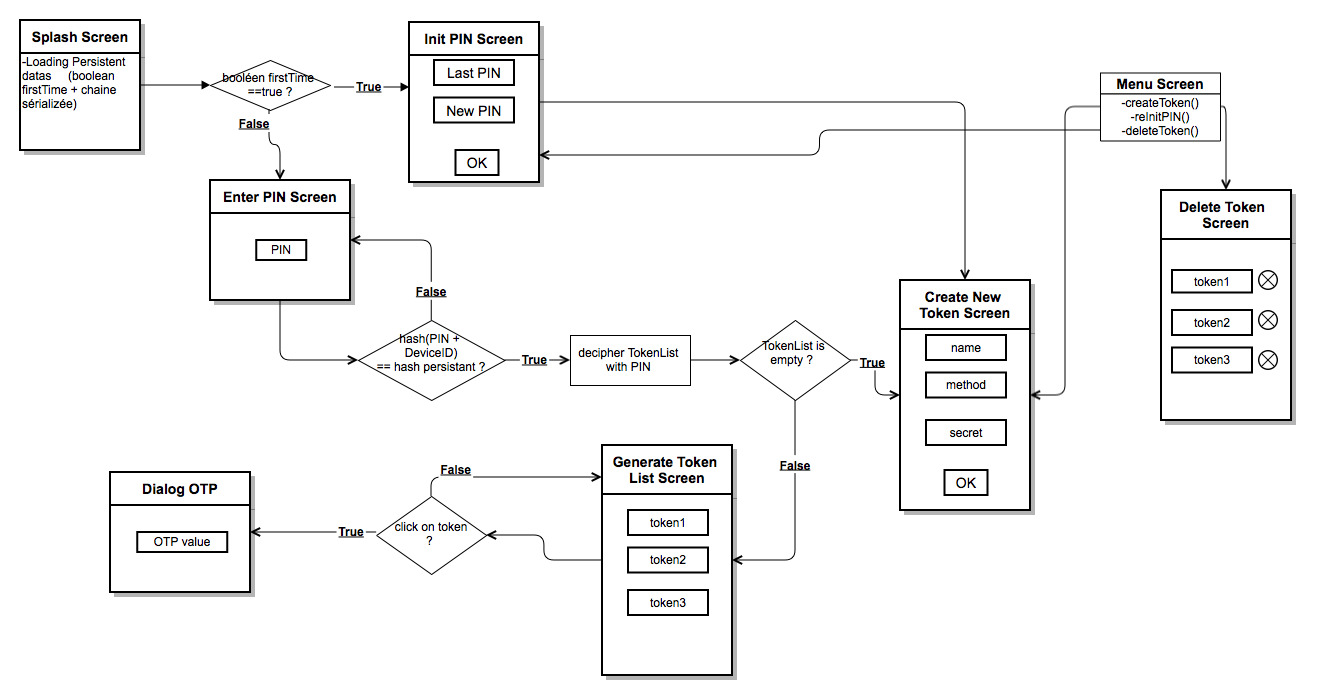
\includegraphics[width=\textwidth]{../graphics/uml_android_token.jpg}

\subsection{Générateur d'OTP}
Les implémentations retenues après études des RFC sont TOTP et HOTP. TOTP
n'étant qu'une variante d'HOTP seul un générateur d'HOTP sera programmé.
On fera varier ses paramètres afin d'obtenir un générateur de TOTP.
    \subsubsection{Rôle}
        Le rôle de cette partie du projet est de générer des mots de passe jetables
à partir d'un secret, d'un compteur et une longueur. 

Pour générer des mots de passe selon le protocole TOTP on passera le temps UTC
divisé par une période en tant que compteur.

    \subsubsection{Services offerts}
    Ce module fournit toute une librairie de génération de mot de passe jetable en fonction du type d’OTP souhaité (TOTP,HOTP).

On y trouve la fonction principale :
\begin{itemize}
\item OTPGenerator.generer()
\end{itemize}

\newpage
Cette fonction utilise nos fonctions utilitaires :
\begin{enumerate}
\item hmacSha1(ISecret key, long count)
\item truncate(byte[] bytes)
\item convert(byte[] bytes)
\end{enumerate}


    \subsubsection{Procédé de développement}
       On commencera par implémenter les fonctions utilitaires qui ne seront pas accessible en
dehors du module. Ensuite nous implémenterons la génération d'OTP.

    \subsubsection{Langages de programmation}
        Le langage utilisé sera Java car c'est le langage recommandé pour Android.

    \subsubsection{Taille et complexité}
C'est l'une des parties nouvelles et cruciale du projet. Non seulement car il n'y 
a que peu de moyen de vérifier que le générateur d'OTP fonctionne réellement. Et
qu'il faut en plus être compatible avec les RFC HOTP et TOTP.

%------------------------------------------------------------------------------
\subsection{Le token}
	\subsubsection{Rôle}
	Le but de ce composant est de fournir une interface android à l’utilisateur , lui permettant de s’authentifier et de pouvoir créer, modifier ou supprimer des tokens de génération de mot de passe jetable.
	\subsubsection{Services offerts}
	Ce module permettra à l’utilisateur  de créer ou modifier le  PIN pour sécuriser l’application en affichant l’activité :
\begin{enumerate}
\item SetPINActivity.java
\item PINLoginActivity.java
\end{enumerate}

Il sera aussi possible de créer  ou de supprimer des tokens  à travers l’activité TokenListActivity.java
\subsection{Justification des choix techniques}

\subsubsection{Le langage Java}
    Le langage Java sera utilisé sur les plateformes Android, car bien qu'il soit possible de programmer en C
    sur Android, ce n'est pas recommandé par \verb?Google?
    \footnote{\href{https://developer.android.com/tools/sdk/ndk/index.html}{Android NDK}}.
L’utilisateur pourra enfin générer ces mots de jetables, une fois authentifié, en cliquant sur les tokens précédemment créés.
	\subsubsection{Procédé de développement}
        On commencera par fournir les fonctions minimales du module, c'est à dire la création, la modification  du PIN utilisateur, l'authentification par ce PIN. Viendra ensuite la partie création des tokens, la gestion de ces tokens puis la génération des mots de passe  jetables.
        \subsubsection{Taille et complexité}
        C'est la deuxième partie cruciale et nouvelle du projet, il faut d'abord que l'équipe s'approprie la technologie ensuite il suffira de développer les fonctions que le module doit fournir.
\part*{Architecture dynamique}

\section{Demande de secret}
\subsection{Principe}
Le secret doit être partagé entre le système hôte et le token. Pour déterminer
le secret il faut faire une demande au système hôte. Ce dernier possède une clé
maîtresse qu'il dérivera pour donner une nouvelle clé à l'utilisateur. L'utilisateur
devra entrer le secret lui même sur le token.

\section{Génération d'OTP}
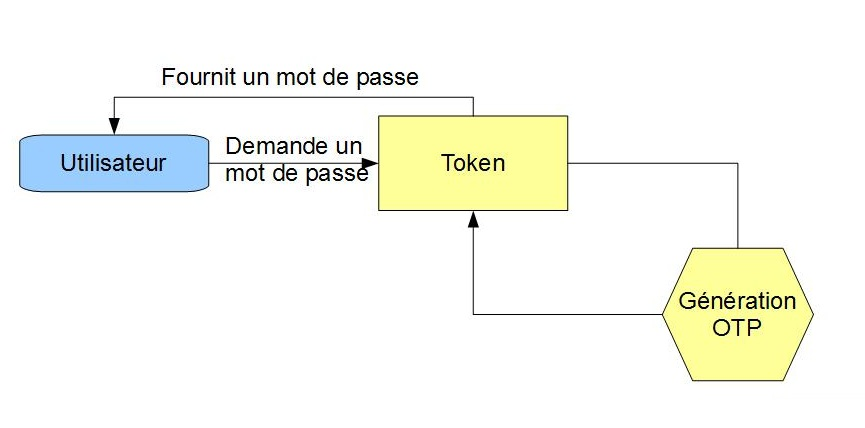
\includegraphics[width=\textwidth]{../graphics/generation.jpg}

\begin{figure}
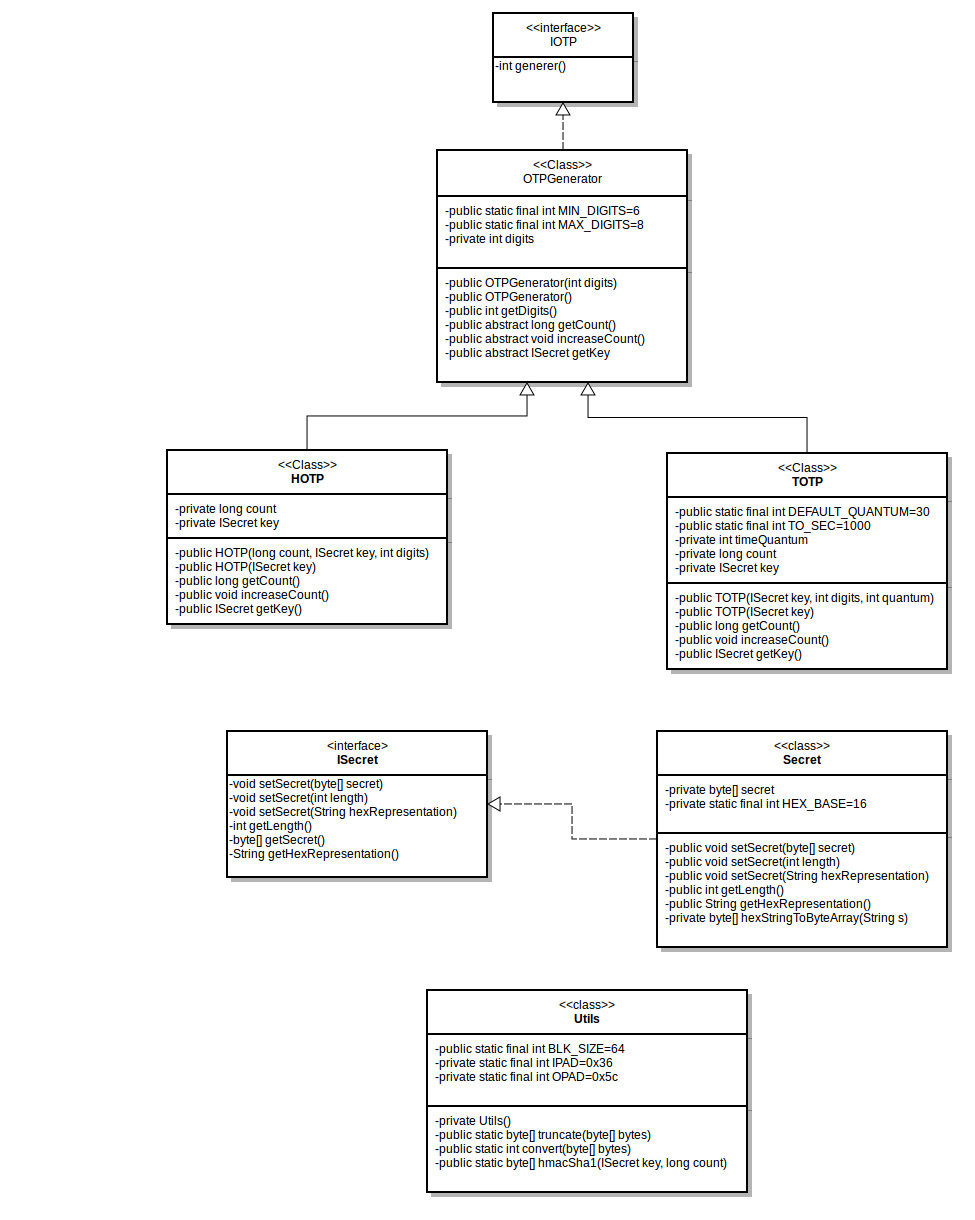
\includegraphics[width=\textwidth]{../graphics/uml_lib.jpg}
\end{figure}



\section{Data Management}
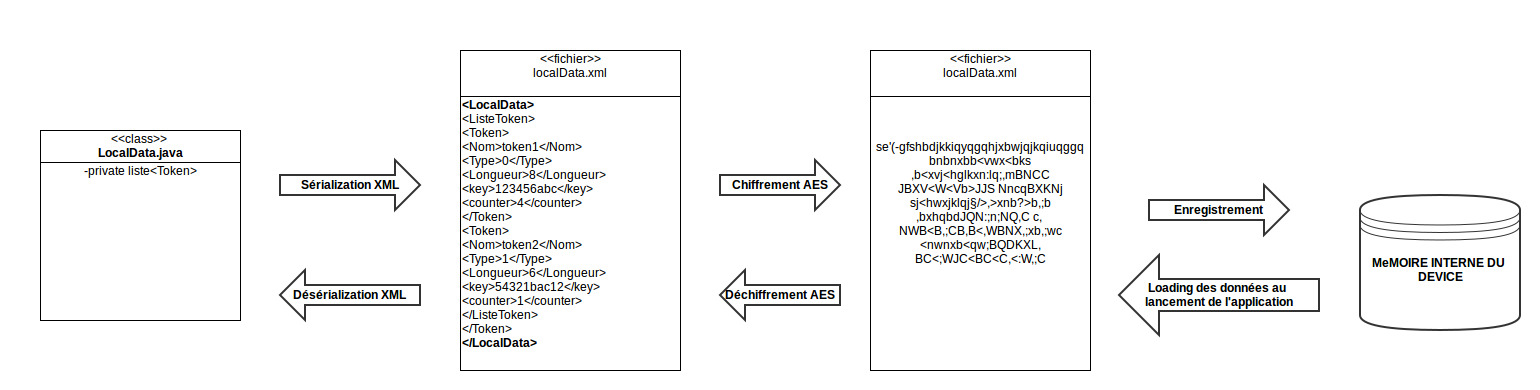
\includegraphics[width=\textwidth]{../graphics/uml_data.jpg}

\section{Use case}
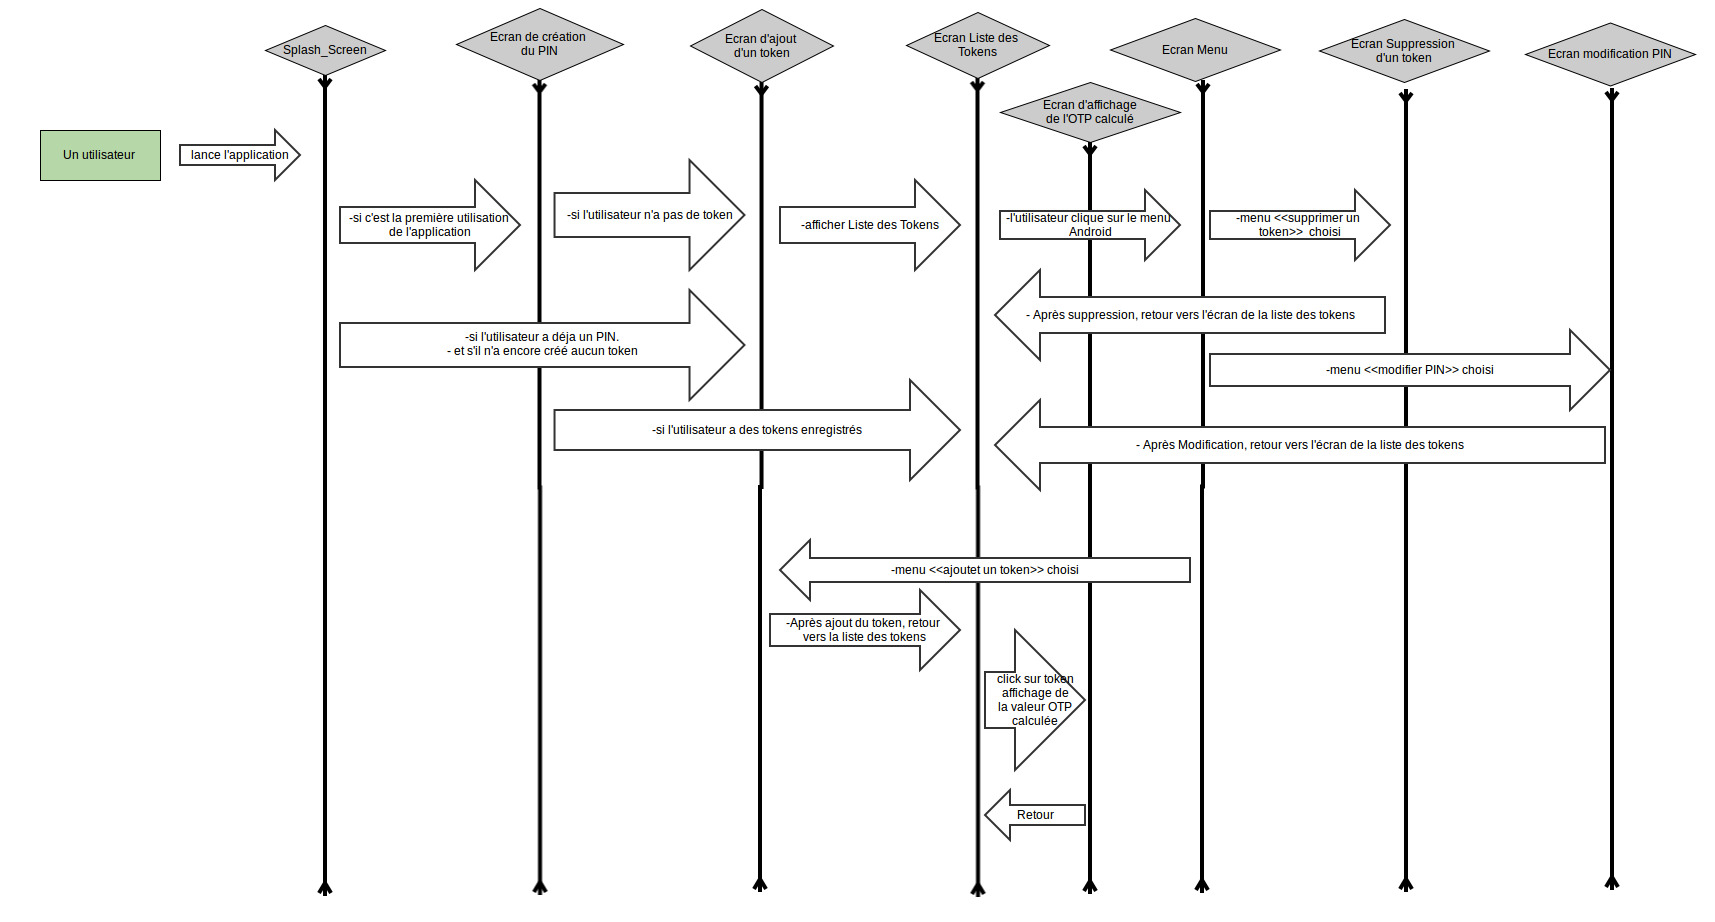
\includegraphics[width=\textwidth]{../graphics/uml_use.jpg}

\end{document}